\section{Déjà Vu}
\begin{marginfigure}
\begin{tikzpicture}
\node [name-dest] (box){%
    \begin{minipage}{0.80\textwidth}
     \begin{itemize}
    \item Tanguy Racine
    \item Clare Tan
    \end{itemize}
    \end{minipage}

};
\node[fancytitle, right=10pt] at (box.north west) {Déjà Vu};
\end{tikzpicture}
\end{marginfigure}

I’d never gone expedition caving with Clare. We had managed to cross paths at X-Ray or on the surface in 2014 and 2015 so we decided to make up for this. We planned to cave after a mid-expedition break in Tolmin spent walking around to the Tolminka gorges and then to the Izvir Tolminke where Will Scott and I got thoroughly drenched. It seemed like exploration in the new shaft series was dying down slightly after the horrors at the bottom of Upside Down chamber so we decided to have a look at the original, older, deeper shaft series, past the infamous Brezno TTT (infamous because it looked wider than most shafts in the system with the exception of Silos and Happy Monday).

It had also not been visited at all during the summer, despite its proximity to the entrance and the relative route-finding ease, but with very good reason until then: we wanted to find our own way down. When had it been last visited? There was also another interesting nexus en route to TTT: Mandare. This crossroads was marked as an open lead on the 2000 survey, and the drawing of it remained unchanged in the 2011 survey, though additions to the deeper series had been made. Why was it so? Finally, we thought it would be good to gain knowledge of the upper part of the original deep series as its passage morphology might give off clues as to where connections between the two shaft series are likely to be found, and whether it had any potential for mid-depth horizontal development as seen in Karstaway. 

From Sejna Soba, the whole of the way to TTT was a basic rift. There were obstacles, of course, how not in a cave of generally small dimensions, fault controlled and full of choss? The odd climb up or down a waterfall, the emergence into the bottom of an aven, navigation in a tight rift. And there were leads. Closest to Sejna Soba was a little carbide arrow pointing the way at a junction, but taking the other option took us to the take-off of a 10 metre deep pitch. This junction is noted on the 2011 survey as an open lead, and admittedly, the pitch is found directly on top of another horizontal branch of the cave. Could it provide another, easier connection? Further on it the impressive Povezava Aven, a 20x20m aven, boulder strewn. It is slighlty slanted however, with the eastern wall dipping towards the west. 10 metres from the floor, a dark recess, 5 metre wide  that could be a window into horizontal passage was spotted. The bolt-climb appears to be a straightforward one, and still very close to the surface. Importantly, Povezava is amongst the easternmost points of Primadona sensu-stricto, and going further east might yield a pathway into much barren mountain so far.



TTT was impressive. If one could find the way to access the pitch from the very top, it would be a good 80m deep, and 20-25m broad throughout. The passage joins in about halfway down the pitch. But where was Mandare? Supposedly the connection between Stara Jama (the old cave) and the Povezava branch, we saw no sign of a passage joining in at right angles to our rift. Though we spotted an aven it was nothing like the drawing on the survey. In all probability, the Povezava branch joins in at the bottom of a pitch, once accessed from the top through Stara Jama. The old way could have been derigged later on. No one had visited the Stara Jama branch, focussed as we were on the new shaft series. 

\begin{marginfigure}
\checkoddpage \ifoddpage \forcerectofloat \else \forceversofloat \fi
\centering
\frame{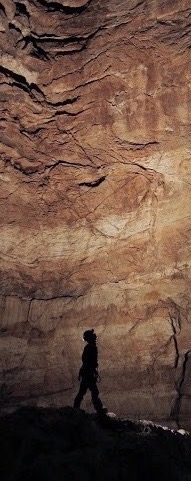
\includegraphics[width=\textwidth]{images/2016/tanguy-dvu-2016/jarv_ttt__1_.jpg}}
\caption{The bottom of TTT (P40) where bus sized boulders accumulated --- Jarvist Frost}
\label{Migsurf}
\end{marginfigure}

After rerigging some of the scaries hangs of TTT (a smaller parallel shaft joined in towards the bottom of the pitch, the wall between the two I assume gradually thinned down to a few feet where the last, loose and rusty hanging rebelay was), we bottomed this might pitch and searched for the way on. On the far, southwestern corner of the almond shaped shaft  we eventually found a small draughting rift leading off. Had we missed an obvious way on? We spotted a small drop that had been rigged, descended and reached another climb down. Seeing no ropes, I was hopeful that this was maybe a small side passage no one went back to, but it clearly went on and the draft was strong. The drop led to an obvious junction of two rifts.

\begin{figure*}[t]
\checkoddpage \ifoddpage \forcerectofloat \else \forceversofloat \fi
\centering
\frame{\includegraphics[width=\textwidth]{"images/2016/tanguy-dvu-2016/ttt_and_below_tr_grade_1"}}
\caption{A grade 1 survey of TTT pitch and the Déjà Vu junction below --- Tanguy Racine}
\label{Grade 1 survey}
\end{figure*}

Clare spotted what she described as a landing cairn, and after placing a beautiful ‘Y’-hang, it became clear that someone had been down. There were abundant footprints on the black-and-brown mottled floor. Further along the rift, downwind past several traverses where drops underneath the false floor got deeper and deeper we reached the ropes. There were many of them, some muddy and attached to homemade hangers, others cleaner with shiny krabs and through-bolts. A set of ropes protected a traverse across a pitch, the other went down.

Since we had not explored the upwind passage at the junction, I proposed that we enter a few metres in the book. Clare agreed so we walked on the mottled floor up into a textbook example of a phreatic tube later turned into a vadose rift. It meandered in a lovely manner, but not for long, soon we were crawling in between mammoth boulders. To our right, there was a small aven which we thought we recognised from before. It seemed we had returned underneath the Brezno TTT rift. As we continued past it underneath another enormous boulder we heard the echo, and drips of a larger chamber beyond, TTT itself not doubt.


\begin{figure*}[t!]
\checkoddpage \ifoddpage \forcerectofloat \else \forceversofloat \fi
\centering
    \begin{subfigure}[t]{0.353\textwidth}
        \centering
         \frame{\includegraphics[width=\linewidth]{"images/2016/tanguy-dvu-2016/jarv_chamber_dejavu__1_".jpg}}
        
        \caption{} \label{Traverse over buckwheat}
    \end{subfigure}
        \hfill
\begin{subfigure}[t]{0.63\textwidth}
\centering
\frame{\includegraphics[width=\linewidth]{"images/2016/tanguy-dvu-2016/jarv_buckwheat__1_".jpg}}
 \caption{}\label{passage in Deja VU}
\end{subfigure}
    \vspace{0cm}
    \begin{subfigure}[t]{\textwidth}
    \centering
       
        \frame{\includegraphics[width=\linewidth]{"images/2016/tanguy-dvu-2016/Jarv_DejaVU__1_".jpg}}
        \caption{} \label{Dejavu}
    \end{subfigure}
    \caption{
    \emph{a} Large boulders have fallen in the chamber in \emph{Déja Vu}.  
     \emph{b} \emph{Ajdovščina} a classic bedding controlled phreatic passage, with subsequent vadose sediment deposited
     \emph{c} The junction between  \emph{Déja Vu} extension and the main TTT branch, where 'leopard spots' are preserved--- Jarvist Frost }
\end{figure*}


Only it was not. It was something else, a drippy, boulder strewn chamber that looked curiously similar to TTT. The water came from a little pitch higher up and the chamber itself had the shape of a kidney. Turning left, the ground rose, and the chamber was dry. Keeping to the left hand wall - we had done an 180° turn at that point, the draught changed from upwind to downwind, and the floor sloped down to a pitch head. Twenty metres deep maybe more. It probably reconnects with the original pitch series, it must, with all the snaking around we can’t have moved off that far. We having rope, drill power and metal work did not bolt down this new pitch. We placed our bets on the already rigged way down Ajdovscina pitch. 

So after a short survey we came back to the bolted pitch head. The traverse was almost an obvious choice, the precedents in Migovec abound: stay high, avoid the water for inevitably disappears down impenetrable cracks, and take your share of glory. The bolts were sound, and the rigging adequate but halfway through I did question my sanity. 20 to 30 metres below, the continuing pitch series awaited. On the far side of the traverse a short 5 metre stoop led to a further pitch head, dry this time. The rope was still dry and mostly clean, the ‘Y’-hang as inviting as any. Clipping into the traverse line I swung over drop, 20m at most and could see that it was a clean hang, landing on a rubble floor. There was still a heap of unused rope there. 

We whizzed down and explored the bottom of the dry pitch. A sloping mud and rubble floor, with the skeleton of a bat, no dry horizontal way on and around a corner, a large window looking into the previous pitch. We decided to use the excess rope to rig down from the window and back into the main way, bypassing the scary bolts. Another beautiful, wide ‘Y’-hang later and I dropped another 10m to reach a ledge, protruding from three sides of a pitch. On the far ledge, a traverse line brought the Slovenians’ way down away from the spray and the unstable boulders. With the water on our side of the ledge we opted to mimic the previous way down. 

Three or four more bolts later I prepared to go down the next drop. The lights couldn’t reach the bottom, but I could see the ropes in place running from one wall to the other like a loose, lonely spider web. Again mimicking the existing rigging I placed two rebelays, and reached a large bouldery ledge. There again there was a profusion of ropes: a rope leading in through the boulders high-up from the last rebelay. On the right hand side of the ledge there were two ropes descending the next section of the pitch. A blue rope which could be accessed by traversing on the broad ledge to the first anchor. And a white rope, a ‘Y’-hang bolted from a rift on the far side of the pitch. Could the rope leading into the boulders find its way to this far rift?  How else to reach it?

When Clare joined up with me, we had a little break and considered our options: we had were precious little bolts left, next to no rope. We didn’t chance using the in-situ rope, instead turned around, with the aim to sort out some of the rigging on the way out. Though we had not found where Jack and Kenneth’s route joined up with the old pitch series, we’d gained the knowledge of the route, its obstacles and gauged the state of the rigging in this forgotten bit of cave. 

Interestingly, we didn’t see any obvious pitch coming in from Déjà Vu as we went down, and looking at the survey, it looks like there is a sizeable distance between Ajdovscina and the pitch head, perhaps as much as 40m horizontally. Can this be the next way down deep?

\name{Tanguy Racine}